\documentclass[a4paper, 11pt]{article}
\usepackage{graphicx}
\usepackage{multicol}
\usepackage{tabularx}
\usepackage{enumitem}
\usepackage[a4paper, margin=1.8cm]{geometry}
\usepackage{listings}
\usepackage{amssymb}
\usepackage{gvv}
\usepackage{gvv-book}
\usepackage{amsmath}
\usepackage{setspace}
\usepackage{caption}

\graphicspath{./figs/}

\begin{document}
\begin{center}
    \huge{EC : ELECTRONICS AND COMMUNICATION ENGINEERING}\\
    \large{EE25BTECH11041 - Naman Kumar}
\end{center}
\section*{General Aptitude (GA)}
\begin{enumerate}
    \item The strategies that the company \underline{\hspace{2cm}} to sell its products \underline{\hspace{2cm}} house-to-house marketing.
    \begin{enumerate}
        \begin{multicols}{2}
            \item use, includes
            \item uses, include
            \item used, includes
            \item uses, including
        \end{multicols}
    \end{enumerate}
    \hfill{\brak{\text{GATE EC 2019}}}

    \item The boat arrived \underline{\hspace{2cm}} dawn.
    \begin{enumerate}
        \begin{multicols}{4}
            \item in
            \item at
            \item on
            \item under
        \end{multicols}
    \end{enumerate}
    \hfill{\brak{\text{GATE EC 2019}}}

    \item It would take one machine 4 hours to complete a production order and another machine 2 hours to complete the same order. If both machines work simultaneously at their respective constant rates, the time taken to complete the same order is \underline{\hspace{2cm}} hours.
    \begin{enumerate}
        \begin{multicols}{4}
            \item 2/3
            \item 3/4
            \item 4/3
            \item 7/3
        \end{multicols}
    \end{enumerate}
    \hfill{\brak{\text{GATE EC 2019}}}

    \item Five different books \brak{P, Q, R, S, T} are to be arranged on a shelf. The books R and S are to be arranged first and second, respectively from the right side of the shelf. The number of different orders in which P, Q and T may be arranged is
    \begin{enumerate}
        \begin{multicols}{4}
            \item 2
            \item 6
            \item 12
            \item 120
        \end{multicols}
    \end{enumerate}
    \hfill{\brak{\text{GATE EC 2019}}}

    \item When he did not come home, she \underline{\hspace{2cm}} him lying dead on the roadside somewhere.
    \begin{enumerate}
        \begin{multicols}{2}
            \item concluded
            \item looked
            \item notice
            \item pictured
        \end{multicols}
    \end{enumerate}
    \hfill{\brak{\text{GATE EC 2019}}}

    \item Four people are standing in a line facing you. They are Rahul, Mathew, Seema and Lohit. One is an engineer, one is a doctor, one a teacher and another a dancer. You are told that:
    \begin{enumerate}[label=\arabic*.]
        \item Mathew is not standing next to Seema
        \item There are two people standing between Lohit and the engineer
        \item Rahul is not a doctor
        \item The teacher and the dancer are standing next to each other
        \item Seema is turning to her right to speak to the doctor standing next to her
    \end{enumerate}
    Who among them is an engineer?
    \begin{enumerate}
        \begin{multicols}{2}
            \item Seema
            \item Lohit
            \item Rahul
            \item Mathew
        \end{multicols}
    \end{enumerate}
    \hfill{\brak{\text{GATE EC 2019}}}

    \item The bar graph in Panel (a) shows the proportion of male and female illiterates in 2001 and 2011. The proportions of males and females in 2001 and 2011 are given in Panel (b) and (c), respectively. The total population did not change during this period. The percentage increase in the total number of literates from 2001 to 2011 is
    \begin{figure}[H]
        \centering
        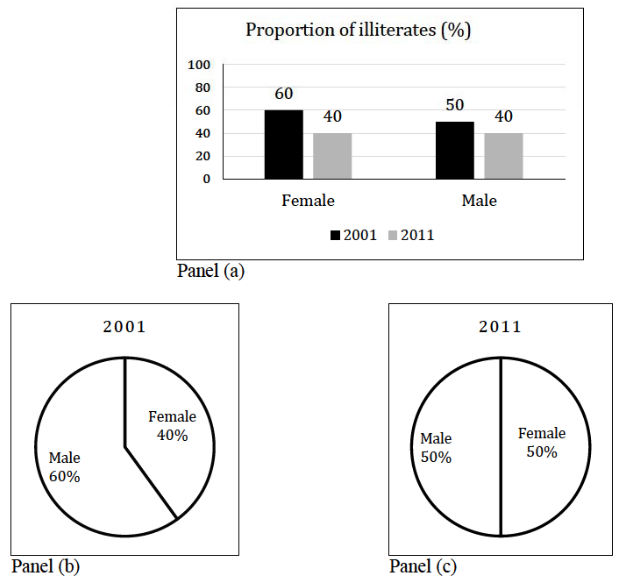
\includegraphics[width=0.8\columnwidth]{figs/GA_Q7.png}
        \caption*{}
        \label{fig:q7}
    \end{figure}
    \begin{enumerate}
        \begin{multicols}{4}
            \item 30.43
            \item 33.43
            \item 34.43
            \item 35.43
        \end{multicols}
    \end{enumerate}
    \hfill{\brak{\text{GATE EC 2019}}}

    \item "Indian history was written by British historians extremely well documented and researched, but not always impartial. History had to serve its purpose: Everything was made subservient to the glory of the Union Jack. Latter-day Indian scholars presented a contrary picture."\\From the text above, we can infer that:\\Indian history written by British historians
    \begin{enumerate}
        \item was well documented and not researched but was always biased
        \item was not well documented and researched and was always biased
        \item was well documented and researched but was sometimes biased
        \item was not well documented and researched and was sometimes biased
    \end{enumerate}
    \hfill{\brak{\text{GATE EC 2019}}}

    \item Two design consultants, P and Q, started working from 8 AM for a client. The client budgeted a total of USD 3000 for the consultants. P stopped working when the hour hand moved by 210 degrees on the clock. Q stopped working when the hour hand moved by 240 degrees. P took two tea breaks of 15 minutes each during her shift, but took no lunch break. Q took only one lunch break for 20 minutes, but no tea breaks. The market rate for consultants is USD 200 per hour and breaks are not paid. After paying the consultants, the client shall have USD \underline{\hspace{2cm}} remaining in the budget.
    \begin{enumerate}
        \begin{multicols}{4}
            \item 000.00
            \item 166.67
            \item 300.00
            \item 433.33
        \end{multicols}
    \end{enumerate}
    \hfill{\brak{\text{GATE EC 2019}}}

    \item Five people P, Q, R, S and T work in a bank. P and Q don't like each other but have to share an office till T gets a promotion and moves to the big office next to the garden. R, who is currently sharing an office with T wants to move to the adjacent office with S, the handsome new intern. Given the floor plan, what is the current location of Q, R and T? \brak{O= Office, WR = Washroom}
    \begin{enumerate}
        \begin{multicols}{2}
            \item 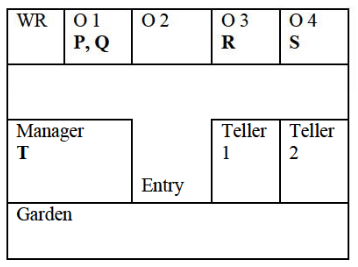
\includegraphics[width=0.9\columnwidth]{figs/GA_Q10A.png}
            \item 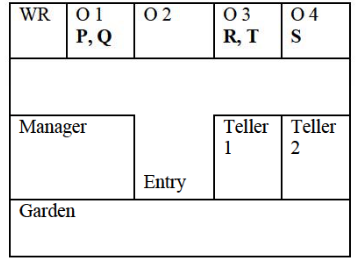
\includegraphics[width=0.9\columnwidth]{figs/GA_Q10B.png}
            \item 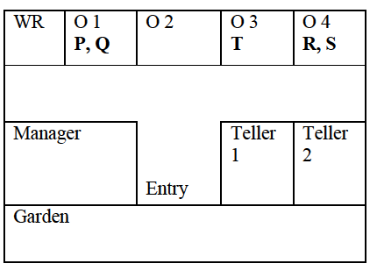
\includegraphics[width=0.9\columnwidth]{figs/GA_Q10C.png}
            \item 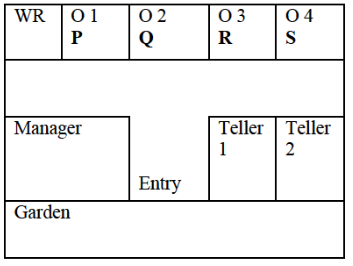
\includegraphics[width=0.9\columnwidth]{figs/GA_Q10D.png}
        \end{multicols}
    \end{enumerate}
    \hfill{\brak{\text{GATE EC 2019}}}
\end{enumerate}

\section*{Electronics and Communication Engineering \brak{EC}}

\begin{enumerate}

    
    \item Which one of the following functions is analytic over the entire complex plane?

    \begin{enumerate}
        \begin{multicols}{2}
            \item $\ln\brak{z}$
            \item $e^{1/z}$
            \item $\frac{1}{1-z}$
            \item $\cos\brak{z}$
        \end{multicols}
    \end{enumerate}

    \hfill{\brak{\text{GATE EC 2019}}}

    \item The families of curves represented by the solution of the equation
    \[
    \frac{dy}{dx}=-\brak{\frac{x}{y}}^{n}
    \]
    for $n=-1$ and $n=+1$, respectively, are
    \begin{enumerate}
        \begin{multicols}{2}
            \item Parabolas and Circles
            \item Circles and Hyperbolas
            \item Hyperbolas and Circles
            \item Hyperbolas and Parabolas
        \end{multicols}
    \end{enumerate}

    \hfill{\brak{\text{GATE EC 2019}}}

    \item Let $H\brak{z}$ be the z-transform of a real-valued discrete-time signal $h[n]$. If $P\brak{z}=H\brak{z}H\brak{\frac{1}{z}}$ has a zero at $z=\frac{1}{2}+\frac{1}{2}j$ and $P\brak{z}$ has a total of four zeros, which one of the following plots represents all the zeros correctly?
    \begin{enumerate}
        \begin{multicols}{2}
            \item 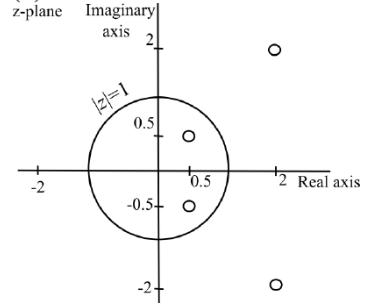
\includegraphics[width=0.9\columnwidth]{figs/q3A.png}
            \item 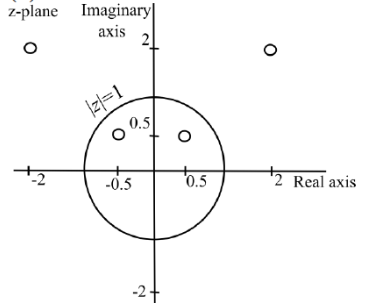
\includegraphics[width=0.9\columnwidth]{figs/q3B.png}
            \item 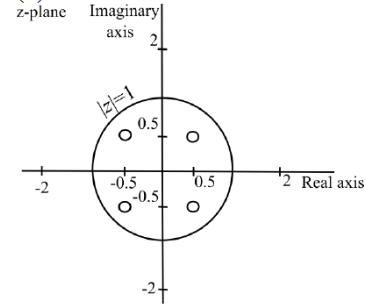
\includegraphics[width=0.9\columnwidth]{figs/q3C.png}
            \item 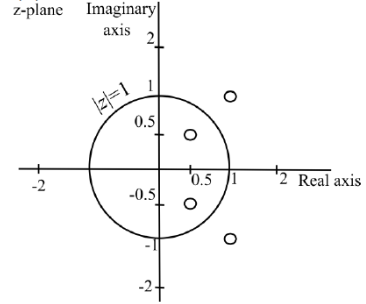
\includegraphics[width=0.9\columnwidth]{figs/q3D.png}
        \end{multicols}
    \end{enumerate}

    \hfill{\brak{\text{GATE EC 2019}}}

    \item Consider the two-port resistive network shown in the figure. When an excitation of $5$ V is applied across Port 1, and Port 2 is shorted, the current through the short circuit at Port 2 is measured to be $1$ A \brak{\text{see (a) in the figure}}.\\Now, if an excitation of $5$ V is applied across Port 2, and Port 1 is shorted \brak{\text{see (b) in the figure}}, what is the current through the short circuit at Port 1?
    
    \begin{figure}[H]
        \centering
        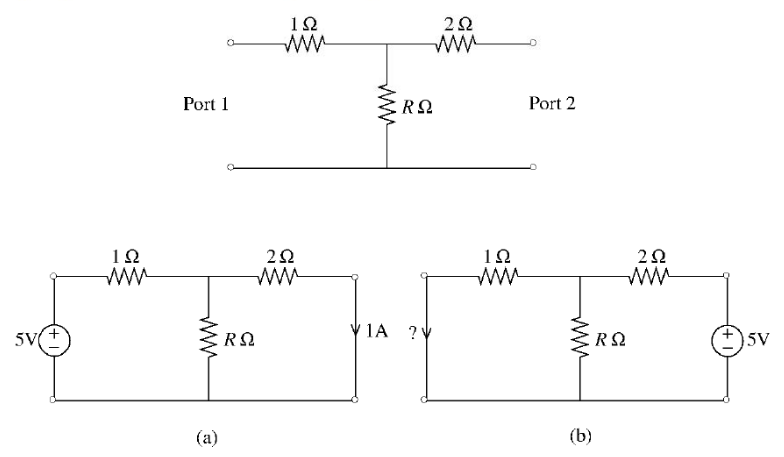
\includegraphics[width=0.8\columnwidth]{figs/q4.png}
        \caption*{}
        \label{fig:q4}
    \end{figure}
    
    \begin{enumerate}
        \begin{multicols}{4}
            \item $0.5$ A
            \item $1$ A
            \item $2$ A
            \item $2.5$ A
        \end{multicols}
    \end{enumerate}

    \hfill{\brak{\text{GATE EC 2019}}}

    \item Let $Y\brak{s}$ be the unit-step response of a causal system having a transfer function
    \begin{center}
    $G\brak{s}=\frac{3-s}{\brak{s+1}\brak{s+3}}$ 
    \end{center}
    that is, $Y\brak{s}=\frac{G\brak{s}}{s}$. The forced response of the system is
    \begin{enumerate}
        \begin{multicols}{2}
            \item $u\brak{t}-2e^{-t}u\brak{t}+e^{-3t}u\brak{t}$
            \item $2u\brak{t}-2e^{-t}u\brak{t}+e^{-3t}u\brak{t}$
            \item $2u\brak{t}$
            \item $u\brak{t}$
        \end{multicols}
    \end{enumerate}

    \hfill{\brak{\text{GATE EC 2019}}}
    
    \item For an LTI system, the Bode plot for its gain is as illustrated in the figure shown. The number of system poles $N_{p}$ and the number of system zeros $N_{z}$ in the frequency range $1 \text{ Hz} \le f \le 10^{7} \text{ Hz}$ is
    
    \begin{figure}[H]
        \centering
        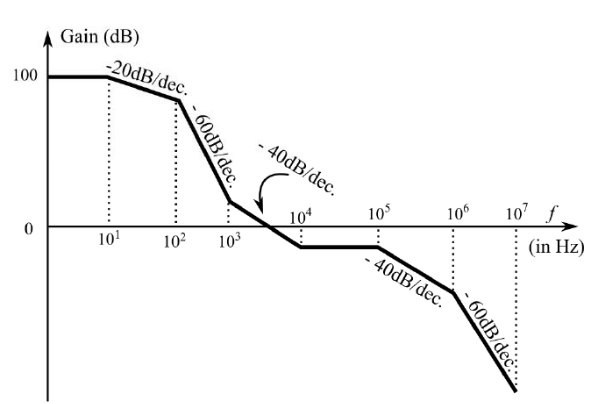
\includegraphics[width=0.5\columnwidth]{figs/q6.png}
        \caption*{}
        \label{fig:q6}
    \end{figure}
    
    \begin{enumerate}
        \begin{multicols}{2}
            \item $N_{p}=5$, $N_{z}=2$
            \item $N_{p}=6$, $N_{z}=3$
            \item $N_{p}=7$, $N_{z}=4$
            \item $N_{p}=4$, $N_{z}=2$
        \end{multicols}
    \end{enumerate}

    \hfill{\brak{\text{GATE EC 2019}}}

    \item A linear Hamming code is used to map 4-bit messages to 7-bit codewords. The encoder mapping is linear. If the message 0001 is mapped to the codeword 0000111, and the message 0011 is mapped to the codeword 1100110, then the message 0010 is mapped to
    \begin{enumerate}
        \begin{multicols}{2}
            \item 0010011
            \item 1100001
            \item 1111000
            \item 1111111
        \end{multicols}
    \end{enumerate}

    \hfill{\brak{\text{GATE EC 2019}}}

    \item Which one of the following options describes correctly the equilibrium band diagram at $T=300$ K of a Silicon $pmn^{+}p^{++}$ configuration shown in the figure?
    \begin{figure}[H]
        \centering
        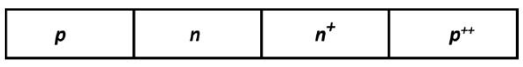
\includegraphics[width=0.5\columnwidth]{figs/q8.png}
        \caption*{}
        \label{fig:q8}
    \end{figure}
    \begin{enumerate}
            \item 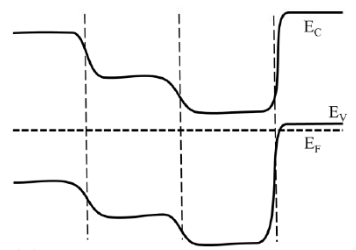
\includegraphics[width=0.9\columnwidth]{figs/q8A.png}
            \item 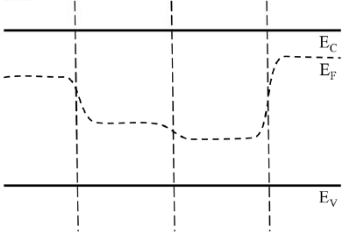
\includegraphics[width=0.9\columnwidth]{figs/q8B.png}
            \item 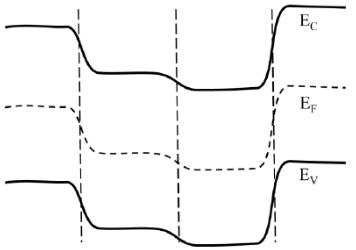
\includegraphics[width=0.9\columnwidth]{figs/q8C.png}
            \item 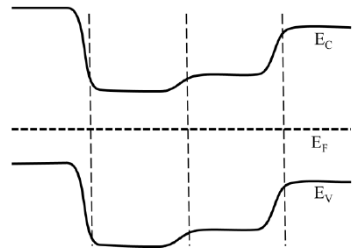
\includegraphics[width=0.9\columnwidth]{figs/q8D.png}
    \end{enumerate}
    
    \hfill{\brak{\text{GATE EC 2019}}}

    \item The correct circuit representation of the structure shown in the figure is
    \begin{figure}[H]
        \centering
        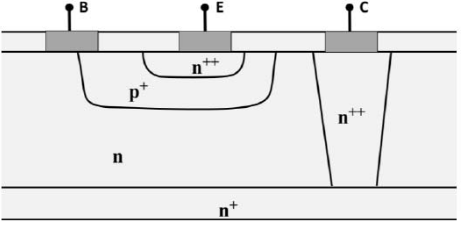
\includegraphics[width=0.5\columnwidth]{figs/q9.png}
        \caption*{}
        \label{fig:q9}
    \end{figure}
    \begin{enumerate}
        \begin{multicols}{2}
            \item 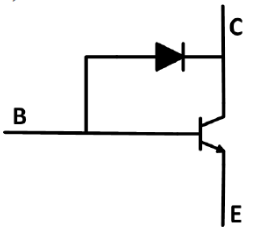
\includegraphics[width=0.9\columnwidth]{figs/q9A.png}
            \item 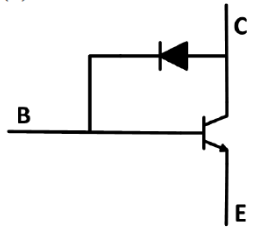
\includegraphics[width=0.9\columnwidth]{figs/q9B.png}
            \item 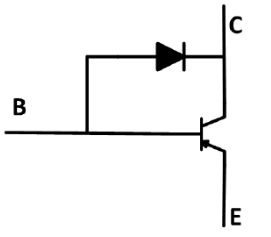
\includegraphics[width=0.9\columnwidth]{figs/q9C.png}
            \item 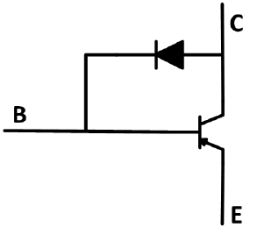
\includegraphics[width=0.9\columnwidth]{figs/q9D.png}
        \end{multicols}
    \end{enumerate}

    \hfill{\brak{\text{GATE EC 2019}}}

    \item The figure shows the high-frequency C-V curve of a MOS capacitor \brak{\text{at $T=300$ K}} with $\Phi_{ms}=0$V and no oxide charges. The flat-band, inversion, and accumulation conditions are represented, respectively, by the points
    
    \begin{figure}[H]
        \centering
        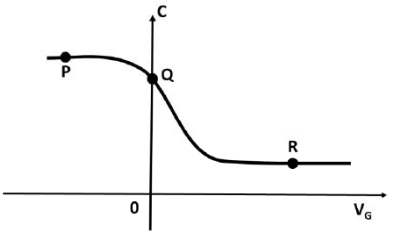
\includegraphics[width=0.4\columnwidth]{figs/q10.png}
        \caption*{}
        \label{fig:q10}
    \end{figure}
    
    \begin{enumerate}
        \item P, Q, R
        \item Q, R, P
        \item R, P, Q
        \item Q, P, R
    \end{enumerate}

    \hfill{\brak{\text{GATE EC 2019}}}

    \item What is the electric flux \brak{$\int\vec{E}\cdot d\hat{a}$} through a quarter-cylinder of height H \brak{\text{as shown in the figure}} due to an infinitely long line charge along the axis of the cylinder with a charge density of Q?
    
    \begin{figure}[H]
        \centering
        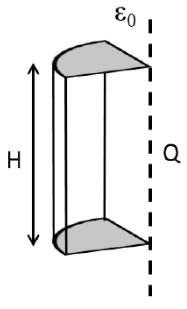
\includegraphics[width=0.3\columnwidth]{figs/q11.png}
        \caption*{}
        \label{fig:q11}
    \end{figure}
    
    \begin{enumerate}
        \begin{multicols}{2}
            \item $\frac{HQ}{\epsilon_{0}}$
            \item $\frac{HQ}{4\epsilon_{0}}$
            \item $\frac{H\epsilon_{0}}{4Q}$
            \item $\frac{4H}{Q\epsilon_{0}}$
        \end{multicols}
    \end{enumerate}

    \hfill{\brak{\text{GATE EC 2019}}}
    
    \item In the table shown, List I and List II, respectively, contain terms appearing on the left-hand side and the right-hand side of Maxwell's equations \brak{\text{in their standard form}}. Match the left-hand side with the corresponding right-hand side.
    
    \begin{table}[H]
    \centering
    \begin{tabular}{|l|l|l|l|}
        \hline
        \multicolumn{2}{|c|}{\textbf{List I}} & \multicolumn{2}{c|}{\textbf{List II}} \\
        \hline
        1 & $\nabla \cdot D$ & P & 0 \\
        \hline
        2 & $\nabla \times E$ & Q & $\rho$ \\
        \hline
        3 & $\nabla \cdot B$ & R & $-\frac{\partial B}{\partial t}$ \\
        \hline
        4 & $\nabla \times H$ & S & $J + \frac{\partial D}{\partial t}$ \\
        \hline
    \end{tabular}
    \caption*{}
    \label{tab:q12}
    \end{table}

    \begin{enumerate}
        \item 1-P, 2-R, 3-Q, 4-S
        \item 1-Q, 2-R, 3-P, 4-S
        \item 1-Q, 2-S, 3-P, 4-R
        \item 1-R, 2-Q, 3-S, 4-P
    \end{enumerate}
    
    \hfill{\brak{\text{GATE EC 2019}}}

    \item A standard CMOS inverter is designed with equal rise and fall times \brak{$\beta_{n}=\beta_{p}$}. If the width of the pMOS transistor in the inverter is increased, what would be the effect on the LOW noise margin \brak{$NM_{L}$} and the HIGH noise margin \brak{$NM_{H}$}?
    
    \begin{enumerate}
        \item $NM_{L}$ increases and $NM_{H}$ decreases.
        \item $NM_{L}$ decreases and $NM_{H}$ increases.
        \item Both $NM_{L}$ and $NM_{H}$ increase.
        \item No change in the noise margins.
    \end{enumerate}

    \hfill{\brak{\text{GATE EC 2019}}}

    \item In the circuit shown, what are the values of F for $EN=0$ and $EN=1$, respectively?
    
    \begin{figure}[H]
        \centering
        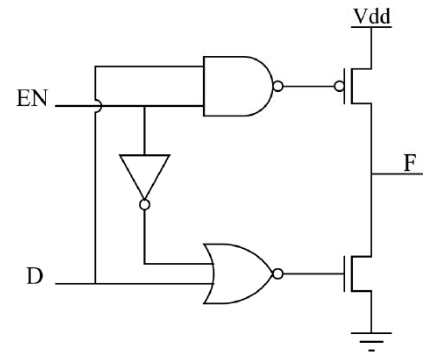
\includegraphics[width=0.5\columnwidth]{figs/q14.png}
        \caption*{}
        \label{fig:q14}
    \end{figure}
    
    \begin{enumerate}
        \item 0 and D
        \item Hi-Z and D
        \item 0 and 1
        \item Hi-Z and $\bar{D}$
    \end{enumerate}
    
    \hfill{\brak{\text{GATE EC 2019}}}
    
    \item In the circuit shown, A and B are the inputs and F is the output. What is the functionality of the circuit?
    
    \begin{figure}[H]
        \centering
        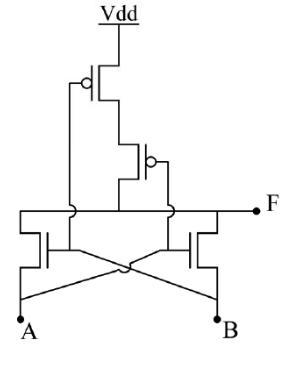
\includegraphics[width=0.3\columnwidth]{figs/q15.png}
        \caption*{}
        \label{fig:q15}
    \end{figure}

    \begin{enumerate}
        \item Latch
        \item XNOR
        \item SRAM Cell
        \item XOR
    \end{enumerate}
    
    \hfill{\brak{\text{GATE EC 2019}}}

    \item The value of the contour integral
    \[
    \frac{1}{2\pi j}\oint\brak{z+\frac{1}{z}}^{2}dz
    \]
    evaluated over the unit circle $|z|=1$ is \underline{\hspace{2cm}}.
    
    \hfill{\brak{\text{GATE EC 2019}}}

    \item The number of distinct eigenvalues of the matrix
    \[
    A = \myvec{2 & 2 & 3 & 3 \\ 0 & 1 & 1 & 1 \\ 0 & 0 & 3 & 3 \\ 0 & 0 & 0 & 2}
    \]
    is equal to \underline{\hspace{2cm}}.
    
    \hfill{\brak{\text{GATE EC 2019}}}
    
    \item If X and Y are random variables such that $E[2X+Y]=0$ and $E[X+2Y]=33$, then $E[X]+E[Y] = $ \underline{\hspace{2cm}}.

    \hfill{\brak{\text{GATE EC 2019}}}

    \item The value of the integral $\int_{0}^{\pi}\int_{y}^{\pi}\frac{\sin x}{x}dx~dy$, is equal to \underline{\hspace{2cm}}.
    
    \hfill{\brak{\text{GATE EC 2019}}}

    \item Let Z be an exponential random variable with mean 1. That is, the cumulative distribution function of Z is given by
    \[
    F_{Z}\brak{x} = 
    \begin{cases}
        1-e^{-x} & \text{if } x \ge 0 \\
        0 & \text{if } x < 0
    \end{cases}
    \]
    Then $Pr\brak{Z>2|Z>1}$, rounded off to two decimal places, is equal to \underline{\hspace{2cm}}.
    
    \hfill{\brak{\text{GATE EC 2019}}}

    \item Consider the signal $f\brak{t}=1+2\cos\brak{\pi t}+3\sin\brak{\frac{2\pi}{3}t}+4\cos\brak{\frac{\pi}{2}t+\frac{\pi}{4}}$, where t is in seconds. Its fundamental time period, in seconds, is \underline{\hspace{2cm}}.
    
    \hfill{\brak{\text{GATE EC 2019}}}

    \item The baseband signal $m\brak{t}$ shown in the figure is phase-modulated to generate the PM signal $\varphi\brak{t}=\cos\brak{2\pi f_{c}t+k~m\brak{t}}$. The time t on the x-axis in the figure is in milliseconds. If the carrier frequency is $f_{c}=50$ kHz and $k=10\pi$, then the ratio of the minimum instantaneous frequency \brak{\text{in kHz}} to the maximum instantaneous frequency \brak{\text{in kHz}} is \underline{\hspace{2cm}} \brak{\text{rounded off to 2 decimal places}}.
    
    \begin{figure}[H]
        \centering
        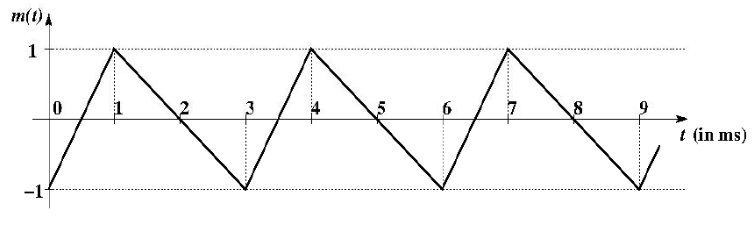
\includegraphics[width=\columnwidth]{figs/q22.png}
        \caption*{}
        \label{fig:q22}
    \end{figure}
    
    \hfill{\brak{\text{GATE EC 2019}}}

    \item Radiation resistance of a small dipole current element of length $l$ at a frequency of 3 GHz is 3 ohms. If the length is changed by 1\%, then the percentage change in the radiation resistance, rounded off to two decimal places, is \underline{\hspace{2cm}}\%.
    
    \hfill{\brak{\text{GATE EC 2019}}}

    \item In the circuit shown, $V_{s}$ is a square wave of period T with maximum and minimum values of 8 V and -10 V, respectively. Assume that the diode is ideal and $R_{1}=R_{2}=50~\ohm$. The average value of $V_{L}$ is \underline{\hspace{2cm}} volts \brak{\text{rounded off to 1 decimal place}}.
    
    \begin{figure}[H]
        \centering
        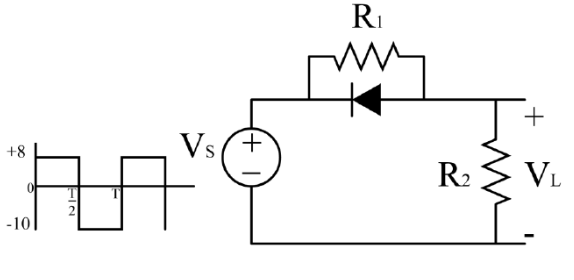
\includegraphics[width=0.6\columnwidth]{figs/q24.png}
        \caption*{}
        \label{fig:q24}
    \end{figure}

    \hfill{\brak{\text{GATE EC 2019}}}
    
    \item In the circuit shown, the clock frequency, i.e., the frequency of the Clk signal, is 12 kHz. The frequency of the signal at $Q_{2}$ is \underline{\hspace{2cm}} kHz.
    
    \begin{figure}[H]
        \centering
        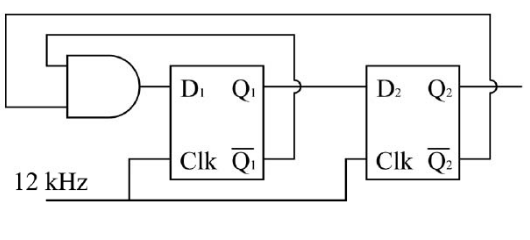
\includegraphics[width=0.6\columnwidth]{figs/q25.png}
        \caption*{}
        \label{fig:q25}
    \end{figure}

    \hfill{\brak{\text{GATE EC 2019}}}
    
    \item Consider a differentiable function $f\brak{x}$ on the set of real numbers such that $f\brak{-1}=0$ and $|f'\brak{x}|\le2$. Given these conditions, which one of the following inequalities is necessarily true for all $x\in[-2,2]$?
    
    \begin{enumerate}
        \item $f\brak{x}\le\frac{1}{2}|x+1|$
        \item $f\brak{x}\le2|x+1|$
        \item $f\brak{x}\le\frac{1}{2}|x|$
        \item $f\brak{x}\le2|x|$
    \end{enumerate}

    \hfill{\brak{\text{GATE EC 2019}}}
    
    \item Consider the line integral
    \[
    \int_{C}\brak{xdy-ydx}
    \]
    the integral being taken in a counterclockwise direction over the closed curve C that forms the boundary of the region R shown in the figure below. The region R is the area enclosed by the union of a $2\times3$ rectangle and a semi-circle of radius 1. The line integral evaluates to
    
    \begin{figure}[H]
        \centering
        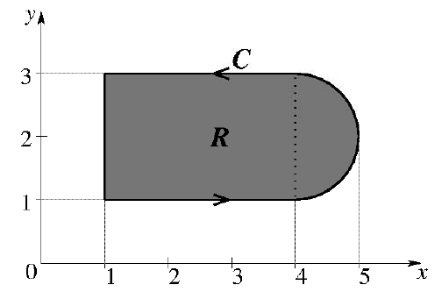
\includegraphics[width=0.5\columnwidth]{figs/q27.png}
        \caption*{}
        \label{fig:q27}
    \end{figure}
    
    \begin{enumerate}
    \begin{multicols}{2}
        \item $6+\pi/2$
        \item $8+\pi$
        \item $12+\pi$
        \item $16+2\pi$
    \end{multicols}
    \end{enumerate}

    \hfill{\brak{\text{GATE EC 2019}}}
    
    \item Consider a six-point decimation-in-time Fast Fourier Transform \brak{FFT} algorithm, for which the signal-flow graph corresponding to $X[1]$ is shown in the figure. Let $W_{6}=exp\brak{-\frac{j2\pi}{6}}$. In the figure, what should be the values of the coefficients $a_{1}$, $a_{2}$, $a_{3}$ in terms of $W_{6}$ so that $X[1]$ is obtained correctly?
    
    \begin{figure}[H]
        \centering
        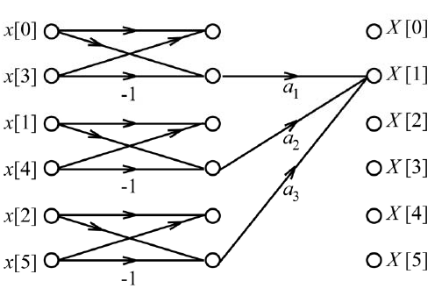
\includegraphics[width=0.8\columnwidth]{figs/q28.png}
        \caption*{}
        \label{fig:q28}
    \end{figure}
    
    \begin{enumerate}
    \begin{multicols}{2}
        \item $a_{1}=-1$, $a_{2}=W_{6}$, $a_{3}=W_{6}^{2}$
        \item $a_{1}=1$, $a_{2}=W_{6}^{2}$, $a_{3}=W_{6}$
        \item $a_{1}=1$, $a_{2}=W_{6}$, $a_{3}=W_{6}^{2}$
        \item $a_{1}=-1$, $a_{2}=W_{6}^{2}$, $a_{3}=W_{6}$
    \end{multicols}
    \end{enumerate}
    
    \hfill{\brak{\text{GATE EC 2019}}}

    \item It is desired to find a three-tap causal filter which gives zero signal as an output to an input of the form
    \[
    x[n]=c_{1}exp\brak{-\frac{j\pi n}{2}}+c_{2}exp\brak{\frac{j\pi n}{2}}
    \]
    where $c_{1}$ and $c_{2}$ are arbitrary real numbers. The desired three-tap filter is given by
    $h[0]=1$, $h[1]=a$, $h[2]=b$ and $h[n]=0$ for $n<0$ or $n>2$. What are the values of the filter taps a and b if the output is $y[n]=0$ for all n, when $x[n]$ is as given above?
    
    \begin{figure}[H]
        \centering
        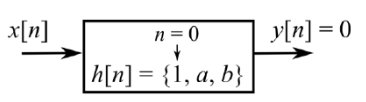
\includegraphics[width=0.7\columnwidth]{figs/q29.png}
        \caption*{}
        \label{fig:q29}
    \end{figure}

    \begin{enumerate}
        \item $a=1$, $b=1$
        \item $a=0$, $b=-1$
        \item $a=-1$, $b=1$
        \item $a=0$, $b=1$
    \end{enumerate}
    
    \hfill{\brak{\text{GATE EC 2019}}}
    
    \item In the circuit shown, if $v\brak{t}=2 \sin\brak{1000 t}$ volts, $R=1$ k$\ohm$ and $C=1$ $\mu$F, then the steady-state current $i\brak{t}$, in milliamperes \brak{mA}, is
    
    \begin{figure}[H]
        \centering
        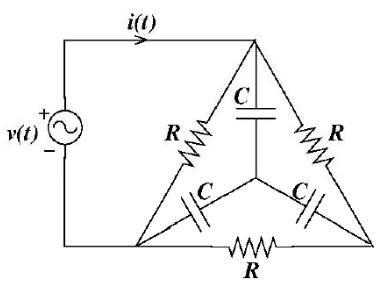
\includegraphics[width=0.5\columnwidth]{figs/q30.png}
        \caption*{}
        \label{fig:q30}
    \end{figure}
    
    \begin{enumerate}
        \item $\sin\brak{1000 t} + \cos\brak{1000 t}$
        \item $2\sin\brak{1000 t} + 2\cos\brak{1000 t}$
        \item $3\sin\brak{1000 t} + \cos\brak{1000 t}$
        \item $\sin\brak{1000 t} + 3\cos\brak{1000 t}$
    \end{enumerate}
    
    \hfill{\brak{\text{GATE EC 2019}}}
    
    \item Consider a causal second-order system with the transfer function
    \[
    G\brak{s}=\frac{1}{1+2s+s^{2}}
    \]
    with a unit-step $R\brak{s}=\frac{1}{s}$ as an input. Let $C\brak{s}$ be the corresponding output. The time taken by the system output $c\brak{t}$ to reach 94\% of its steady-state value $\lim_{t\rightarrow\infty}c\brak{t}$, rounded off to two decimal places, is
    
    \begin{enumerate}
    \begin{multicols}{4}
        \item 5.25
        \item 4.50
        \item 3.89
        \item 2.81
    \end{multicols}
    \end{enumerate}
    
    \hfill{\brak{\text{GATE EC 2019}}}

    \item The block diagram of a system is illustrated in the figure shown, where $X\brak{s}$ is the input and $Y\brak{s}$ is the output. The transfer function $H\brak{s}=\frac{Y\brak{s}}{X\brak{s}}$ is
    
    \begin{figure}[H]
        \centering
        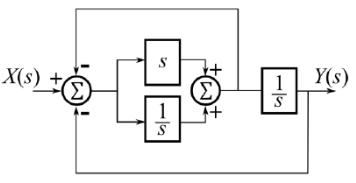
\includegraphics[width=0.7\columnwidth]{figs/q32.png}
        \caption*{}
        \label{fig:q32}
    \end{figure}
    
    \begin{enumerate}
        \item $H\brak{s}=\frac{s^{2}+1}{s^{3}+s^{2}+s+1}$
        \item $H\brak{s}=\frac{s^{2}+1}{s^{3}+2s^{2}+s+1}$
        \item $H\brak{s}=\frac{s+1}{s^{2}+s+1}$
        \item $H\brak{s}=\frac{s^{2}+1}{2s^{2}+1}$
    \end{enumerate}
    
    \hfill{\brak{\text{GATE EC 2019}}}
    
    \item Let the state-space representation of an LTI system be $\dot{x}\brak{t}=A x\brak{t}+B u\brak{t}$, $y\brak{t}=C x\brak{t}+d u\brak{t}$ where A, B, C are matrices, d is a scalar, $u\brak{t}$ is the input to the system, and $y\brak{t}$ is its output. Let $B=[0 \ 0 \ 1]^{T}$ and $d=0$. Which one of the following options for A and C will ensure that the transfer function of this LTI system is
    \[
    H\brak{s}=\frac{1}{s^{3}+3s^{2}+2s+1}?
    \]
    
    \begin{enumerate}
        \item $A=\myvec{0 & 1 & 0 \\ 0 & 0 & 1 \\ -1 & -2 & -3}$ and $C=[1 \ 0 \ 0]$
        \item $A=\myvec{0 & 1 & 0 \\ 0 & 0 & 1 \\ -3 & -2 & -1}$ and $C=[1 \ 0 \ 0]$
        \item $A=\myvec{0 & 1 & 0 \\ 0 & 0 & 1 \\ -1 & -2 & -3}$ and $C=[0 \ 0 \ 1]$
        \item $A=\myvec{0 & 1 & 0 \\ 0 & 0 & 1 \\ -3 & -2 & -1}$ and $C=[0 \ 0 \ 1]$
    \end{enumerate}
    
    \hfill{\brak{\text{GATE EC 2019}}}
    
    \item A single bit, equally likely to be 0 and 1, is to be sent across an additive white Gaussian noise \brak{AWGN} channel with power spectral density $N_{0}/2$. Binary signaling, with $0\mapsto p\brak{t}$ and $1\mapsto q\brak{t}$, is used for the transmission, along with an optimal receiver that minimizes the bit-error probability.\\Let $\varphi_{1}\brak{t}$, $\varphi_{2}\brak{t}$ form an orthonormal signal set.\\If we choose $p\brak{t}=\varphi_{1}\brak{t}$ and $q\brak{t}=-\varphi_{1}\brak{t}$, we would obtain a certain bit-error probability $P_{b}$.\\If we keep $p\brak{t}=\varphi_{1}\brak{t}$, but take $q\brak{t}=\sqrt{E}\varphi_{2}\brak{t}$, for what value of E would we obtain the same bit-error probability $P_{b}$?
    \begin{enumerate}
    \begin{multicols}{2}
        \item 0
        \item 1
        \item 2
        \item 3
    \end{multicols}
    \end{enumerate}
    
    \hfill{\brak{\text{GATE EC 2019}}}
    
    \item The quantum efficiency $\brak{\eta}$and responsivity \brak{R} at a wavelength $\lambda$ $\brak{in \mu m}$ in a p-i-n photodetector are related by
    \begin{enumerate}
    \begin{multicols}{2}
        \item $R=\frac{\eta\times\lambda}{1.24}$
        \item $R=\frac{\lambda}{\eta\times1.24}$
        \item $R=\frac{1.24\times\lambda}{\eta}$
        \item $R=\frac{1.24}{\eta\times\lambda}$
    \end{multicols}
    \end{enumerate}
    
    \hfill{\brak{\text{GATE EC 2019}}}
    
    \item Two identical copper wires W1 and W2, placed in parallel as shown in the figure, carry currents I and 2I, respectively, in opposite directions. If the two wires are separated by a distance of 4r, then the magnitude of the magnetic field $\vec{B}$ between the wires at a distance r from W1 is
    
    \begin{figure}[H]
        \centering
        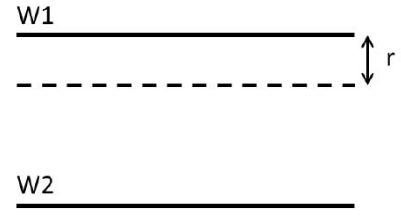
\includegraphics[width=0.4\columnwidth]{figs/q36.png}
        \caption*{}
        \label{fig:q36}
    \end{figure}
    
    \begin{enumerate}
    \begin{multicols}{2}
        \item $\frac{\mu_{0}I}{6\pi r}$
        \item $\frac{6\mu_{0}I}{5\pi r}$
        \item $\frac{5\mu_{0}I}{6\pi r}$
        \item $\frac{\mu_{0}^{2}l^{2}}{2\pi r^{2}}$
    \end{multicols}
    \end{enumerate}
    
    \hfill{\brak{\text{GATE EC 2019}}}
    
    \item The dispersion equation of a waveguide, which relates the wavenumber k to the frequency $\omega$, is
    \[
    k\brak{\omega}=(1/c)\sqrt{\omega^{2}-\omega_{o}^{2}}
    \]
    where the speed of light $c=3\times10^{8}$m/s, and $\omega_{o}$ is a constant. If the group velocity is $2\times10^{8}$m/s, then the phase velocity is
    
    \begin{enumerate}
        \item $1.5\times10^{8}$m/s
        \item $2\times10^{8}$m/s
        \item $3\times10^{8}$m/s
        \item $4.5\times10^{8}$m/s
    \end{enumerate}

    \hfill{\brak{\text{GATE EC 2019}}}
    
    \item In the circuit shown, the breakdown voltage and the maximum current of the Zener diode are 20 V and 60 mA, respectively. The values of $R_{1}$ and $R_{L}$ are 200 $\ohm$ and 1 k$\ohm$, respectively. What is the range of $V_{i}$ that will maintain the Zener diode in the 'on' state?
    
    \begin{figure}[H]
        \centering
        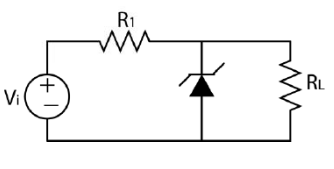
\includegraphics[width=0.6\columnwidth]{figs/q38.png}
        \caption*{}
        \label{fig:q38}
    \end{figure}
    
    \begin{enumerate}
        \item 22 V to 34 V
        \item 24 V to 36 V
        \item 18 V to 24 V
        \item 20 V to 28 V
    \end{enumerate}

    \hfill{\brak{\text{GATE EC 2019}}}
    
    \item The state transition diagram for the circuit shown is
    
    \begin{figure}[H]
        \centering
        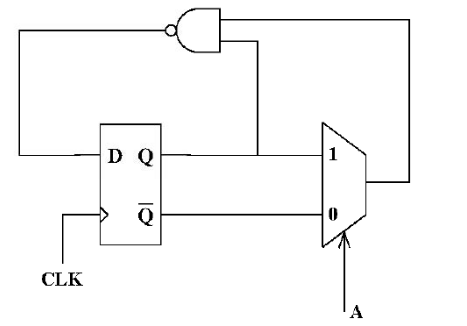
\includegraphics[width=0.5\columnwidth]{figs/q39.png}
        \caption*{}
        \label{fig:q39}
    \end{figure}
    
    \begin{enumerate}
            \item 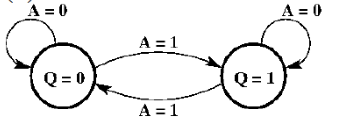
\includegraphics[width=0.5\columnwidth]{figs/q39A.png}
            \item 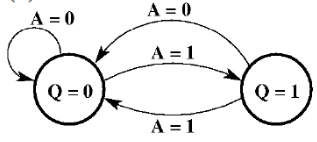
\includegraphics[width=0.5\columnwidth]{figs/q39B.png}
            \item 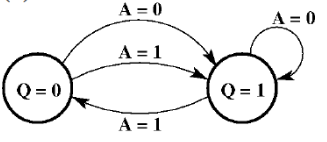
\includegraphics[width=0.5\columnwidth]{figs/q39C.png}
            \item 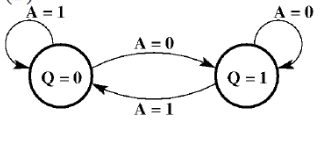
\includegraphics[width=0.5\columnwidth]{figs/q39D.png}
        
    \end{enumerate}

    \hfill{\brak{\text{GATE EC 2019}}}
    
    \item In the circuits shown, the threshold voltage of each nMOS transistor is 0.6 V. Ignoring the effect of channel length modulation and body bias, the values of Vout1 and Vout2, respectively, in volts, are
    
    \begin{figure}[H]
        \centering
        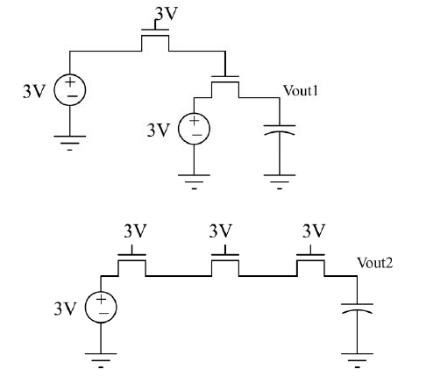
\includegraphics[width=0.5\columnwidth]{figs/q40.png}
        \caption*{}
        \label{fig:q40}
    \end{figure}
    
    \begin{enumerate}
    \begin{multicols}{4}
        \item 1.8 and 1.2
        \item 2.4 and 2.4
        \item 1.8 and 2.4
        \item 2.4 and 1.2
    \end{multicols}
    \end{enumerate}
    
    \hfill{\brak{\text{GATE EC 2019}}}

    \item The RC circuit shown below has a variable resistance $R\brak{t}$ given by the following expression:
    \[
    R\brak{t}=R_{0}\brak{1-\frac{t}{T}} \text{ for } 0\le t<T
    \]
    where $R_{0}=1~\Omega$ and $C=1~F$. We are also given that $T=3~R_{0}C$ and the source voltage is $V_{s}=1$ V. If the current at time $t=0$ is 1 A, then the current $I\brak{t}$, in amperes, at time $t=T/2$ is \underline{\hspace{2cm}} \brak{\text{rounded off to 2 decimal places}}.
    
    \begin{figure}[H]
        \centering
        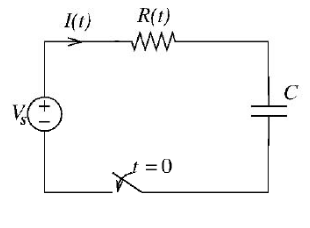
\includegraphics[width=0.4\columnwidth]{figs/q41.png}
        \caption*{}
        \label{fig:q41}
    \end{figure}

    \hfill{\brak{\text{GATE EC 2019}}}
    
    \item Consider a unity feedback system, as in the figure shown, with an integral compensator $\frac{K}{s}$ and open-loop transfer function
    \[
    G\brak{s}=\frac{1}{s^{2}+3s+2}
    \]
    where $K>0$. The positive value of K for which there are exactly two poles of the unity feedback system on the j$\omega$ axis is equal to \underline{\hspace{2cm}} \brak{\text{rounded off to two decimal places}}.
    
    \begin{figure}[H]
        \centering
        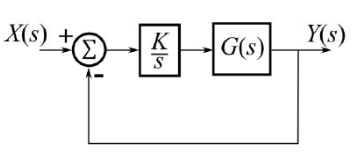
\includegraphics[width=0.6\columnwidth]{figs/q42.png}
        \caption*{}
        \label{fig:q42}
    \end{figure}
    
    \hfill{\brak{\text{GATE EC 2019}}}

    \item Consider the homogeneous ordinary differential equation
    \[
    x^{2}\frac{d^{2}y}{dx^{2}}-3x\frac{dy}{dx}+3y=0, \quad x>0
    \]
    with $y\brak{x}$ as a general solution. Given that $y\brak{1}=1$ and $y\brak{2}=14$, the value of $y\brak{1.5}$, rounded off to two decimal places, is \underline{\hspace{2cm}}.
    
    \hfill{\brak{\text{GATE EC 2019}}}
    
    \item Let $h[n]$ be a length-7 discrete-time finite impulse response filter, given by
    \begin{align*}
        h[0] &= 4, \\
        h[1] &= 3, \quad h[2]=2, \quad h[3]=1, \\
        h[-1] &= -3, \quad h[-2]=-2, \quad h[-3]=-1,
    \end{align*}
    and $h[n]$ is zero for $|n|\ge4$. A length-3 finite impulse response approximation $g[n]$ of $h[n]$ has to be obtained such that\\\[E\brak{h,g}=\int_{-\pi}^{\pi}|H\brak{e^{j\omega}}-G\brak{e^{j\omega}}|^{2}d\omega\]\\is minimized, where $H\brak{e^{j\omega}}$ and $G\brak{e^{j\omega}}$ are the discrete-time Fourier transforms of $h[n]$ and $g[n]$, respectively. For the filter that minimizes $E\brak{h,g}$, the value of $10g[-1]+g[1]$, rounded off to 2 decimal places, is \underline{\hspace{2cm}}.
    
    \hfill{\brak{\text{GATE EC 2019}}}
    
    \item Let a random process $Y\brak{t}$ be described as $Y\brak{t}=h\brak{t}*X\brak{t}+Z\brak{t}$, where $X\brak{t}$ is a white noise process with power spectral density $S_{x}\brak{f}=5~W/Hz$. The filter $h\brak{t}$ has a magnitude response given by $|H\brak{f}|=0.5$ for $-5\le f\le5$ and zero elsewhere. $Z\brak{t}$ is a stationary random process, uncorrelated with $X\brak{t}$, with power spectral density as shown in the figure. The power in $Y\brak{t}$ in watts, is equal to \underline{\hspace{2cm}} W \brak{\text{rounded off to two decimal places}}.
    
    \begin{figure}[H]
        \centering
        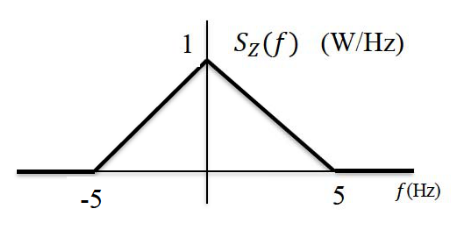
\includegraphics[width=0.6\columnwidth]{figs/q45.png}
        \caption*{}
        \label{fig:q45}
    \end{figure}
    
    \hfill{\brak{\text{GATE EC 2019}}}
    
    \item A voice signal $m\brak{t}$ is in the frequency range 5 kHz to 15 kHz. The signal is amplitude-modulated to generate an AM signal $f\brak{t}=A\brak{1+m\brak{t}}\cos~2\pi f_{c}t$, where $f_{c}=600$ kHz. The AM signal $f\brak{t}$ is to be digitized and archived. This is done by first sampling $f\brak{t}$ at 1.2 times the Nyquist frequency, and then quantizing each sample using a 256-level quantizer. Finally, each quantized sample is binary coded using K bits, where K is the minimum number of bits required for the encoding. The rate, in Megabits per second \brak{\text{rounded off to 2 decimal places}}, of the resulting stream of coded bits is \underline{\hspace{2cm}} Mbps.
    
    \hfill{\brak{\text{GATE EC 2019}}}
    
    \item A random variable X takes values -1 and +1 with probabilities 0.2 and 0.8, respectively. It is transmitted across a channel which adds noise N, so that the random variable at the channel output is $Y=X+N$. The noise N is independent of X, and is uniformly distributed over the interval [-2, 2]. The receiver makes a decision
    \[
    \hat{X}=
    \begin{cases}
        -1, & \text{if } Y\le\theta\\
        +1, & \text{if } Y>\theta.
    \end{cases}
    \]
    where the threshold $\theta\in[-1,1]$ is chosen so as to minimize the probability of error $Pr[\hat{X}\ne X]$. The minimum probability of error, rounded off to 1 decimal place, is \underline{\hspace{2cm}}.
    
    \hfill{\brak{\text{GATE EC 2019}}}
    
    \item A Germanium sample of dimensions $1~cm\times1$ cm is illuminated with a 20 mW, 600 nm laser light source as shown in the figure. The illuminated sample surface has a 100 nm of loss-less Silicon dioxide layer that reflects one-fourth of the incident light. From the remaining light, one-third of the power is reflected from the Silicon dioxide-Germanium interface, one-third is absorbed in the Germanium layer, and one-third is transmitted through the other side of the sample. If the absorption coefficient of Germanium at 600 nm is $3\times10^{4}cm^{-1}$ and the bandgap is 0.66 eV, the thickness of the Germanium layer, rounded off to 3 decimal places, is \underline{\hspace{2cm}} $\mu$m.
    
    \begin{figure}[H]
        \centering
        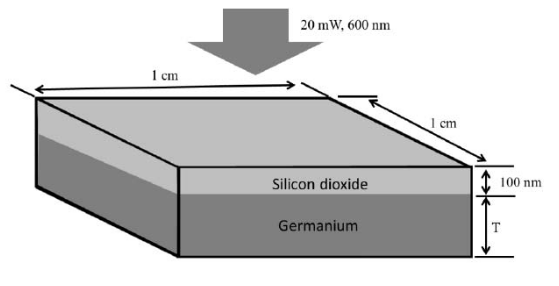
\includegraphics[width=0.6\columnwidth]{figs/q48.png}
        \caption*{}
        \label{fig:q48}
    \end{figure}
    
    \hfill{\brak{\text{GATE EC 2019}}}
    
    \item In an ideal pn junction with an ideality factor of 1 at $T=300~K$, the magnitude of the reverse-bias voltage required to reach 75\% of its reverse saturation current, rounded off to 2 decimal places, is \underline{\hspace{2cm}} mV.
    
    \hfill{\brak{\text{GATE EC 2019}}}
    
    \item Consider a long-channel MOSFET with a channel length 1 $\mu$m and width 10 $\mu$m. The device parameters are acceptor concentration $N_{A}=5\times10^{16}cm^{-3}$, electron mobility $\mu_{n}=800~cm^{2}/V-s$, oxide capacitance/area $C_{ox}=3.45\times10^{-7}F/cm^{2}$, threshold voltage $V_{T}=0.7~V$. The drain saturation current $\brak{I_{Dsat}} $for a gate voltage of 5 V is \underline{\hspace{2cm}} mA \brak{\text{rounded off to two decimal places}}.
    
    \hfill{\brak{\text{GATE EC 2019}}}
    
    \item A rectangular waveguide of width w and height h has cut-off frequencies for $TE_{10}$ and $TE_{11}$ modes in the ratio 1: 2. The aspect ratio $w/h$, rounded off to two decimal places, is \underline{\hspace{2cm}}.
    
    \hfill{\brak{\text{GATE EC 2019}}}
    
    \item In the circuit shown, $V_{s}$ is a 10 V square wave of period, $T=4$ ms with $R=500~\Omega$ and $C=10~\mu F$. The capacitor is initially uncharged at $t=0$, and the diode is assumed to be ideal. The voltage across the capacitor $\brak{V_{c}}$ at 3 ms is equal to \underline{\hspace{2cm}} volts \brak{\text{rounded off to one decimal place}}.
    
    \begin{figure}[H]
        \centering
        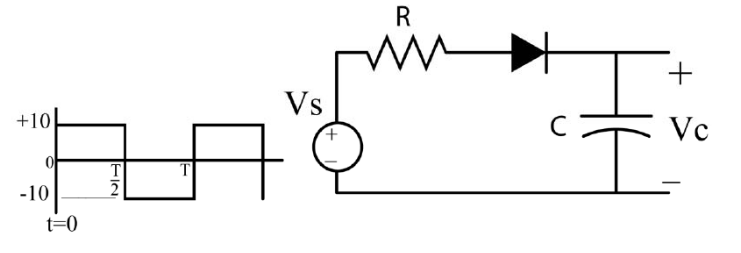
\includegraphics[width=0.6\columnwidth]{figs/q52.png}
    \end{figure}
    
    \hfill{\brak{\text{GATE EC 2019}}}
    
    \item A CMOS inverter, designed to have a mid-point voltage $V_{I}$ equal to half of $V_{dd}$, as shown in the figure, has the following parameters:
    \begin{align*}
        V_{dd}&=3~V \\
        \mu_{n}C_{ox}&=100~\mu A/V^{2}; V_{tn}=0.7~V \text{ for nMOS} \\
        \mu_{p}C_{ox}&=40~\mu A/V^{2}; |V_{tp}|=0.9~V \text{ for pMOS}
    \end{align*}
    The ratio of $\brak{\frac{W}{L}}_{n}$ to $\brak{\frac{W}{L}}_{p}$ is equal to \underline{\hspace{2cm}} \brak{\text{rounded off to 3 decimal places}}.
    
    \begin{figure}[H]
        \centering
        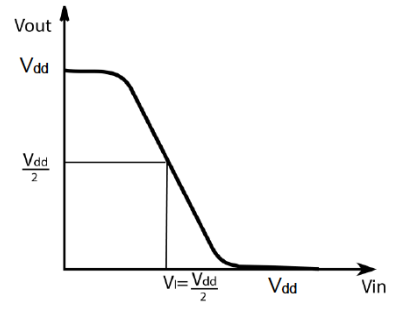
\includegraphics[width=0.5\columnwidth]{figs/q53.png}
        \caption*{}
        \label{fig:q53}
    \end{figure}
    
    \hfill{\brak{\text{GATE EC 2019}}}

    \item In the circuit shown, the threshold voltages of the PMOS \brak{$|V_{tp}|$} and nMOS \brak{$V_{tn}$} transistors are both equal to 1 V. All the transistors have the same output resistance $r_{ds}$ of 6 M$\ohm$. The other parameters are listed below:
    \begin{align*}
        \mu_{n}C_{ox}&=60~\mu A/V^{2}; \brak{\frac{W}{L}}_{nMos}=5 \\
        \mu_{p}C_{ox}&=30~\mu A/V^{2}; \brak{\frac{W}{L}}_{PMOS}=10
    \end{align*}
    $\mu_{n}$ and $\mu_{p}$ are the carrier mobilities, and $C_{ox}$ is the oxide capacitance per unit area. Ignoring the effect of channel length modulation and body bias, the gain of the circuit is \underline{\hspace{2cm}} \brak{\text{rounded off to 1 decimal place}}.
    
    \begin{figure}[H]
        \centering
        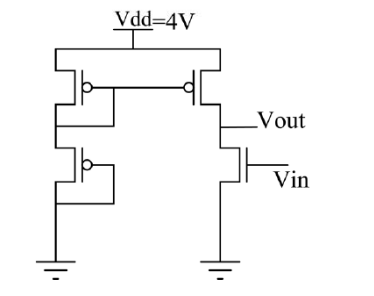
\includegraphics[width=0.4\columnwidth]{figs/q54.png}
        \caption*{}
        \label{fig:q54}
    \end{figure}

    \hfill{\brak{\text{GATE EC 2019}}}

    \item In the circuit shown, $V_{1}=0$ and $V_{2}=V_{dd}$. The other relevant parameters are mentioned in the figure. Ignoring the effect of channel length modulation and the body effect, the value of $I_{out}$ is \underline{\hspace{2cm}} mA \brak{\text{rounded off to 1 decimal place}}.
    
    \begin{figure}[H]
        \centering
        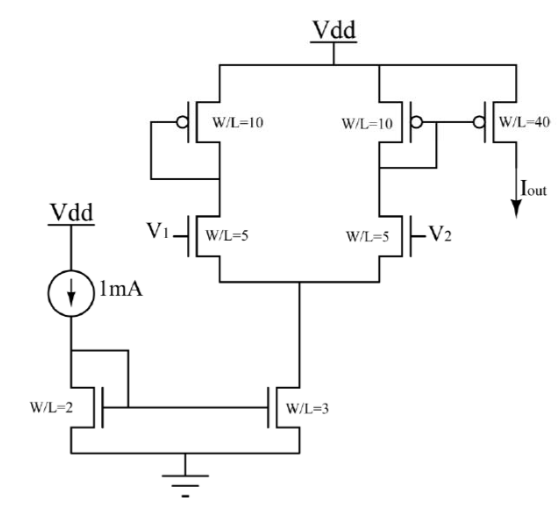
\includegraphics[width=0.6\columnwidth]{figs/q55.png}
        \caption*{}
        \label{fig:q55}
    \end{figure}
    
    \hfill{\brak{\text{GATE EC 2019}}}

\end{enumerate}

\end{document}

